\documentclass[11pt,letterpaper,boxed,noheader]{pset}

\usepackage[margin=0.75in]{geometry}
\usepackage{ulem}

\begin{document}

    \problemlist{PHYS051 HW14}
    \begin{center}
        T1.19; T1.24; *T1.25; T1.26; T1.27; T1.29; T1.34
    \end{center}
    
    
    \begin{problem} [T1.19]
        Express the complex number $z_1 = (\sqrt{3}+i)/2$ in the form $re^{i\phi}$. What about $z_2 = (1 + \sqrt{3}i)/2$? If these complex numbers are the probability amplitudes for photons to be detected, what is the probability in each case?
    \end{problem}
    \newpage
    
    \begin{problem} [T1.24]
        \begin{enumerate}
            \item [a.] Show that the probability of a photon of wavelength $\lambda$ being reflected from a thin layer of glass of thickness $d$ at normal incidence is given by 
            \[ P = 0.16 \text{sin}^2 (2 \pi d / \lambda')\]
            where $\lambda'$ is the wavelength of light in glass, i.e., $\lambda' = \lambda/n$, where $n$ is the index of refraction of glass. \textit{Note:} In this calculation assume that the magnitude of the amplitude for reflection from the top or the bottom surface of the glass is 0.2 and that there is an additional phase change of $\pi$ in the reflection from the top surface. Also assume that the amplitudes that arise from multiple reflections between the top and bottom surface of the glass can be neglected in your calculation. Given the result of Problem 1.23, it is okay to approximate the magnitude of the amplitude for transmission as one. \textit{Hint:} What extra distance does light travel in being reflected from the bottom surface relative to the top surface?
            \item [b.] In \textit{QED: The Strange Theory of Light and Matter} Feynman states that as the thickness of a thin layer of glass increases from zero thickness, the probability of reflection first reaches a value of 0.16 when the thickness of the layer of glass is 5 millionths of an inch. What index of refraction is being assumed? Assume $\lambda = 706$ nm. 
            \item [c.] What is the minimum value of $d$ necessary to produce zero reflection?
        \end{enumerate}
    \end{problem}
    \newpage
    
    \begin{problem} [*T1.25]
        Suppose that a thin film of acetone (index of refraction $n$ = 1.25) of thickness $d$ is coating a thick plate of glass (index of refraction = 1.50). Take the magnitude of the amplitude for reflection of a photon from the top or the bottom surface of the acetone at normal incidence to be $r$ and assume that there is an additional phase change of $\pi$ in the reflection from the top \textit{and} the bottom surface of the acetone, since at each of these surfaces light is passing from a medium with a lower index of refraction to one with a higher index of refraction. Calculate the probability that a photon of wavelength $\lambda$ is reflected. Assume that amplitudes that involve multiple reflections at the bottom surface of the film can be neglected in your calculation. Express your answer in terms $\lambda$ and $r$ as well as the thickness $d$ and the index of refraction $n$ of the acetone. What is the minimum thickness of the coating necessary to produce zero reflection? \textit{Note:} For the air-acetone and acetone- glass surfaces $r \cong 0.1$.
    \end{problem}
    \newpage
    
    \begin{problem} [T1.26]
        Assume that the first beam splitter at A in the Mach-Zehnder interferometer (Fig. 1.23) is a "third-silvered mirror," that is, a mirror that reflects one-third the light and transmits two-thirds. The two mirrors at B and C reflect 100\% of the light, and the second beam splitter at D is a traditional half-silvered mirror that reflects one-half the light and transmits one-half. The probability of detecting a photon in either photomultiplier $PM_1$ or $PM_2$ varies with the position of the movable mirror, say mirror B. Determine the maximum probability and the minimum probability of obtaining a count in, say, $PM_1$. What is the visibility
        \[V = \frac{P_{max}-P_{min}}{P_{max}+P_{min}}\]
        of the interference fringes, where $P_{max}$ and $P_{min}$ are the maximum and minimum probabilities, respectively, that a photon is counted by the detector, as the position of the movable mirror varies? \textit{Note:} In the experiment of Aspect et al. described in Section 1.5 the visibility of the fringes is $0.987 \pm 0.005$.
    \end{problem}
    
    \begin{figure} [ht]
        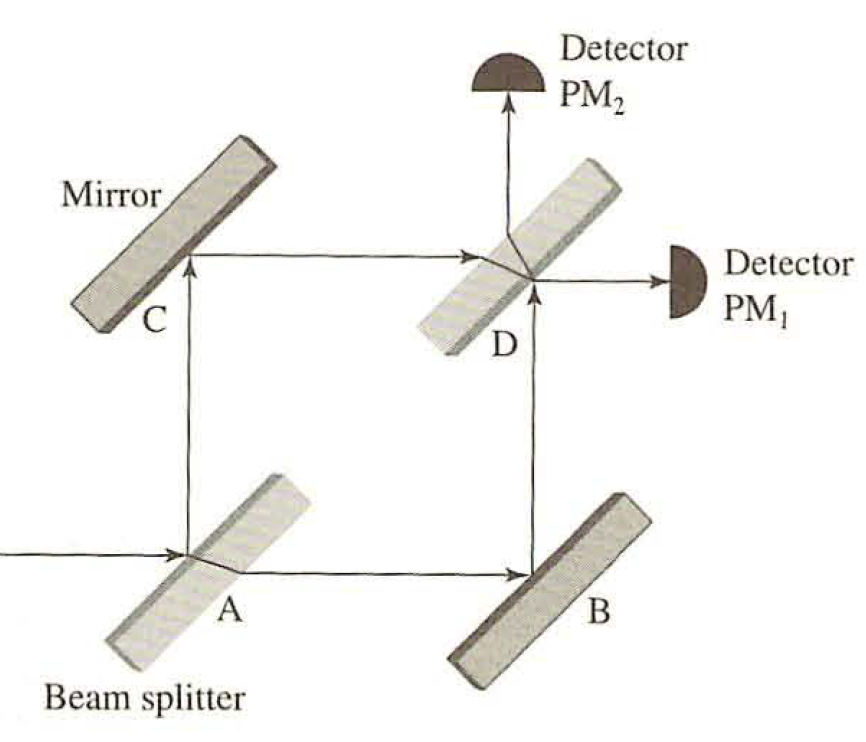
\includegraphics[width=150px]{HW14Images/T1-26.png}
    \end{figure}
    \newpage
    
    \begin{problem} [T1.27]
        Figure 1.43 shows a Michelson interferometer with a movable mirror $M_1$, a fixed mirror $M_2$, and a beam splitter $M_S$ which is a half-silvered mirror that transmits one-half the light and reflects one-half the light incident upon it independent of the direction of the light. The source emits monochromatic light of wavelength $\lambda$. There are two paths that light can follow from the source to the detector, as indicated in the figure. Note that path 1 includes travel from the beam splitter $M_s$, to the movable mirror $M_1$ and back to the beam splitter, while path 2 includes travel from the beam splitter $M_s$ to the fixed mirror $M_2$ and back to the beam splitter. Assume the beam splitter introduces a phase change of $\pi$ for light that follows path 1 from the source to the detector relative to light that follows path 2 from the source to the detector. Also assume the mirrors $M_1$ and $M_2$ reflect 100\% of the light incident upon them and the photodetector PM (a photomultiplier) is 100\% efficient as well.
        
        \begin{enumerate}
            \item [a.] Use the principles of quantum mechanics to determine the probability that a photon entering the interferometer is detected by the photodetector. Express your answer in terms of lengths $l_1, l_2,$ and $\lambda$.
            \item [b.] Find an expression for $l_1$ in terms of $l_2$ and $\lambda$ such that there is 100\% probability that the photon is detected by the photodetector. 
            \item [c.] Suppose that the movable mirror is shifted upward by a distance $\lambda/6$ from the position(s) that you determined in part \textit{(b)}. Find the probability that the photon is detected at the photodetector in this case.
        \end{enumerate}
    \end{problem}
    
    \begin{figure} [ht]
        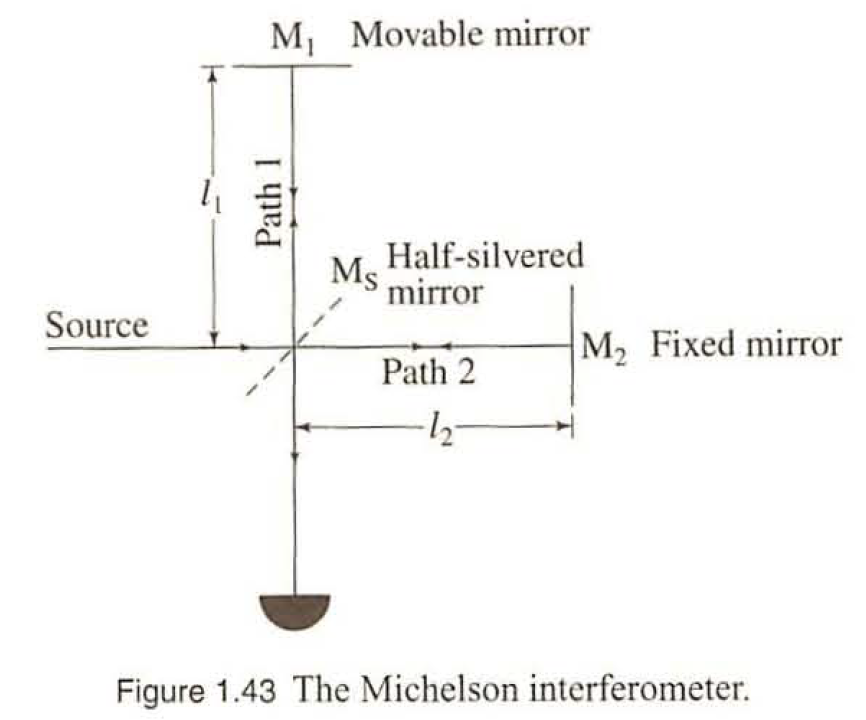
\includegraphics[width=175px]{HW14Images/T1-27.png}
    \end{figure}
    \newpage
    
    \begin{problem} [T1.29]
        Suppose that the two very narrow slits (widths $\ll \lambda$) in the double-slit experiment are not the same width and that the probability amplitude for a photon of wavelength $\lambda$ to strike a photomultiplier centered at particular point P in the detection plane that makes an angle $\theta$ with the horizontal from one of the slits is larger by a factor of $\sqrt{2}$ than for the other slit. Determine the visibility
        \[V = \frac{P_{max} - P_{min}}{P_{max}+P_{min}}\]
        of the interference fringes, where $P_{max}$ is the maximum probability and $P_{min}$ is the minimum probability that a photon is detected. 
    \end{problem}
    \newpage
    
    \begin{problem} [T1.34]
        Starting from first principles, show that the probability of a photon of wavelength $\lambda$ jits a photomultiplier centered on a point P in the detection plane that makes an angle $\theta$ with the horizontal for a grating composed of three very narrow slits each separated by a distance $d$ is given by 
        \[ \text{Prob} = r^2(1+4\text{cos}\phi + 4\text{cos}^2\phi) \]
        where $r^2$ is the probability that the photon would strike the photomultiplier with a single slit open and $\phi=kd \text{sin} \theta = 2 \pi d \text{sin} \theta/\lambda$.
    \end{problem}
\end{document}